\chapter{Timing attacks}
	\index{Timing attacks}Come anticipato nel capitolo precedente, approfondiremo adesso la tipologia di attacchi basati sul tempo focalizzandoci maggiormente su quelli che hanno come obiettivo la cache del processore. 
	
	L'idea di base che sta sotto i timing attacks è quella che l'esecuzione di un determinato programma, al variare delle operazioni che vengono eseguite e al variare degli input, impiega tempi diversi per portare a termine il proprio compito.
	
	\begin{figure}
		\begin{center}
			\lstinputlisting[language=Java]{code/timingBase.txt}
			\caption{Esempio di una funzione attaccabile tramite un timing attack}
			\label{fig:timingBase}
		\end{center}
	\end{figure}
	
	Ad esempio il codice in \cref{fig:timingBase} se fatto girare con la stringa ("passwordToBeStolen") impiegherà un tempo maggiore rispetto allo stesso programma fatto girare con la stringa ("foo"). Nel primo caso infatti verrà scansionata tutta la stringa mentre nel secondo caso si interromperà immediatamente. Questa informazione può essere utilizzata dall'attaccante per capire la stringa esatta. Per portare questo concetto al livello che ci interessa vediamo prima delle nozioni fondamentali sulla cache del processore. 
	
	\section{La cache del processore}
		Dato che la differenza di velocità tra le memorie e la capacità di calcolo dei processori aumenta sempre di più \cite{hennessy2011computer} la banda del bus di comunicazione e la velocità di accesso alla memoria principale sono diventati un fattore limitante sul throughput generale del processore. Questo collo di bottiglia viene attenuato dall'utilizzo delle cache\index{Cache}.
		
		\subsection{Struttura della cache}
			La cache è un piccolo banco di memoria molto veloce sito all'interno di ogni core che il processore utilizza per immagazzinare i valori delle celle di memoria accedute più recentemente. I processori moderni hanno generalmente due livelli di cache per ogni core (L1 e L2). Considerando che l'accesso alla memoria principale in media impiega dai 50 ai 150 \emph{ns} mentre l'accesso alla cache L1 utilizza un tempo nell'ordine degli 0.3 \emph{ns} si può capire l'enorme differenza di prestazioni che possono essere raggiunte utilizzando questo tipo di memoria.
			
			\begin{figure}
				\begin{center}
					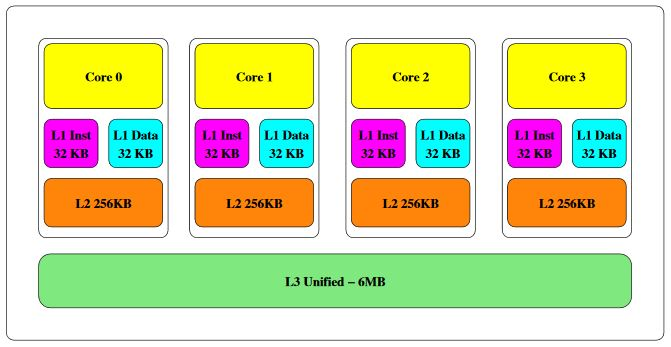
\includegraphics[scale=0.5]{cachei5}
					\caption{Architettura del processore Intel Core i5-3470}
					\label{fig:cachei5}
				\end{center}
			\end{figure}
		
			Nella \ref{fig:cachei5} si può vedere l'architettura del processore quadcore Intel Core i5-3470. La gerarchi delle cache è organizzata in una memoria L1 di 64KB (divisa in 32KB per le istruzioni e 32KB per i dati) ed una memoria L2 da 256KB per ogni core ed un terzo livello chiamato L3 o \ac{LLC} da 6MB comune a tutti e 4 i core.
			
			Andiamo ad analizzare più nel dettaglio le caratteristiche di una singola cache\cite{ge2016survey,yarom2014flush+}.
			
			\subsubsection{Cache lines}
				\index{Cache lines}Per sfruttare la località spaziale le caches sono divise in lines. Una cache line contiene un blocco di Bytes adiacenti (generalmente di dimensione congrua ad una potenza di 2) caricati dalla memoria. Se uno qualunque dei Bytes deve essere rimosso (si parla di \emph{evicting}) per far spazio ad un altro dato, tutta la line viene ricaricata.
				
			\subsubsection{Associatività}
				Teoricamente una qualunque posizione di memoria può essere mappata in una qualunque cache line ed una cache ad \emph{n} lines potrebbe contenere \emph{n} linee qualunque dalla memoria. Questo tipo di cache viene chiamato \emph{fully-associative cache}\index{Fully-associative cache} ed è la migliore in teoria perché può sempre essere usata al massimo delle sue capacità e i cache miss si hanno solamente quando non c'è più spazio libero nella cache. In pratica però questo si traduce in un controllo in parallelo di tutte le linee che aumenta la complessità architetturale e il consumo di energia.
				
				L'estremo opposto è chiamato \emph{direct-mapped cache}\index{Direct-mapped cache}. In questo sistema ogni locazione di memoria può stare in una sola cache line, ben determinata da una funzione di indicizzazione. Due locazioni di memoria che mappano sulla stessa cache line non possono essere immagazzinate contemporaneamente e il loading di una comporta inevitabilmente l'evicting dell'altra. Questo potrebbe portare ad avere dei miss anche con la cache semivuota.
				
				Concretamente viene utilizzata una via di mezzo tra queste due soluzioni chiamata \emph{set-associative cache}\index{Set-associative cache}. La cache viene divisa in \emph{sets} (generalmente di dimensione compresa tra 2 e 24 lines) in cui ogni indirizzo viene controllato in parallelo come in una fully-associative cache. In quale set viene mappato un blocco di memoria viene calcolato come per una direct-mapped cache da una funzione del suo indirizzo. Una cache con \emph{n} line sets viene chiamata \emph{n-way associative}.
				
				Si può notare che le direct-mapped e le fully-associative cache non sono altro che casi particolari di set-associative cache rispettivamente 1-way associative ed N-way associative (dove N è il numero di linee della cache).
				
			\subsubsection{Inclusività}
				Una caratteristica che verrà sfruttata per montare l'attacco è l'\emph{inclusività}\index{Inclusività}. 
				
				Ogni livello superiore di cache contiene un sottoinsieme dei dati contenuti dal livello direttamente inferiore. Per mantenere questa caratteristica, quando viene eseguito un evicting di un dato da un livello inferiore, questo viene rimosso anche da tutti i livelli superiori.
				
			
			
	